\chapter{Images as Functions}

\section{Image}

一张图片 $ f $ 可以看做是 $ \mathbb{R}^2 $ 到 $ \mathbb{R}^M $ 的函数:
\begin{itemize}
    \item $ f(x,y) $ 给出了位置 $ (x,y) $ 的强度
    \item 定义在一个有限的矩形区域内:
    $ f: [a,b] \times [c,d] \rightarrow \mathbb{R}^M $
    \item 像素值:
    \begin{itemize}
        \item \textbf{灰度/强度}: $[0,255]$, 单通道
        \item \textbf{颜色 (RGB)}: $[R, G, B]$, 三通道
    \end{itemize}
\end{itemize}

\textbf{Note:} 图片通常是数字形式 (\textbf{离散化了}).

\section{Image Gradient}
\begin{itemize}
    \item 图像梯度 :
    $$
    \nabla f = \left[\frac{\partial f}{\partial x}, \frac{\partial f}{\partial y}\right]
    $$
    我们实际上使用有限差分来加你计算梯度:
    $$
    \frac{\partial f}{\partial x} \bigg|_{x=x_0} \approx \frac{f(x_0 + 1, y_0) - f(x_0 - 1, y_0)}{2}
    $$
    \item 梯度大小 / 幅度:
    $$
    \|\nabla f\| = \sqrt{\left(\frac{\partial f}{\partial x}\right)^2 + \left(\frac{\partial f}{\partial y}\right)^2}
    $$
    \item 梯度方向:指向强度变化最快的方向。我们可以立即看到梯度和 edge 之间的强相关性。
\end{itemize}

% --- Placeholder for image "VisualizingImageGradient.png" ---
\begin{figure}[htbp]
    \centering
    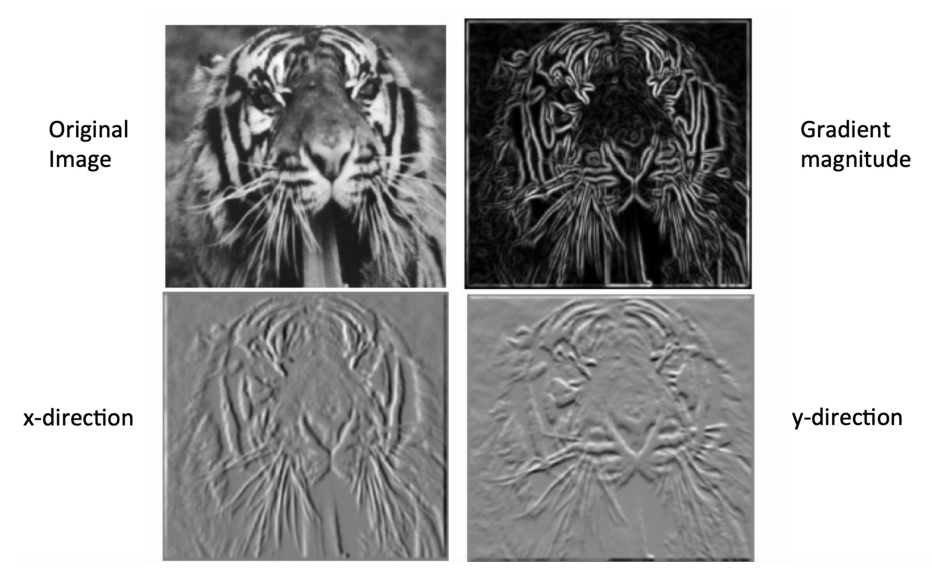
\includegraphics[scale=0.3]{figures/VisualizingImageGradient.png}
    \caption{Visualization of image gradient.}
\end{figure}

\clearpage

\section{Filters}
\begin{itemize}
    \item \textbf{滤波(Filtering)}: 通过组合原始像素值生成新图像的过程,也即滤波是\textbf{选择性保留或去除信号/图像中特定频率成分} 的操作。
    $$
    f[n] \rightarrow \text{System } \mathcal{G} \rightarrow h[n], \quad h = \mathcal{G}(f), \quad h[n] = \mathcal{G}(f)[n]
    $$
    \item \textbf{线性滤波(Linear Filtering)}: 一个系统 $ \mathcal{G} $ 是线性的,如果:
    $$
    \mathcal{G}(\alpha f + \beta g) = \alpha \mathcal{G}(f) + \beta \mathcal{G}(g)
    $$
    \item \textbf{离散卷积(Discrete Convolution)}:
    $$
    (f * g)[n] = \sum_{k=-\infty}^{\infty} f[k] \cdot g[n - k]
    $$
    \item 关键性质:
    \begin{itemize}
        \item \textbf{导数定理}: $$\frac{d}{dt}(f * g) = f * g'$$ 注意这里的 $*$ 是卷积操作不是乘法。
        \item \textbf{卷积定理}: 
        $$
        \mathcal{F}(f * g) = \mathcal{F}(f) \cdot \mathcal{F}(g) \quad \Rightarrow \quad h = \mathcal{F}^{-1}(\mathcal{F}(f) \cdot \mathcal{F}(g))
        $$
        其中,$ \mathcal{F} $ 是傅里叶变换,$ \mathcal{F}^{-1} $ 是傅里叶逆变换。
        
        卷积定理的直观理解就是:在时域中卷积等价于在频域中乘积。

    \end{itemize}
\end{itemize}

% --- Placeholder for image "FourierTransform.png" ---
\begin{figure}[htbp]
    \centering
    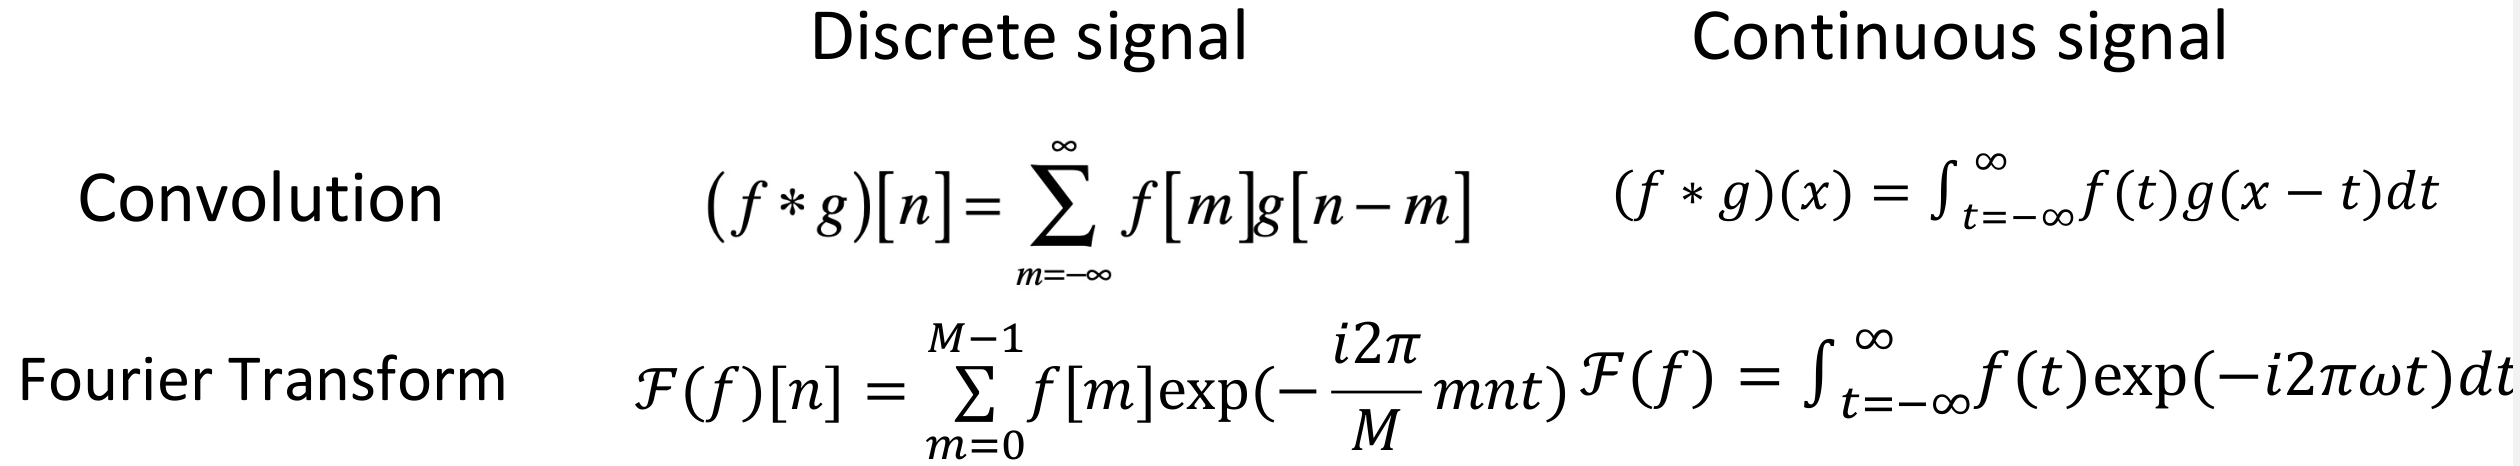
\includegraphics[scale=0.18]{figures/FourierTransform.png}
    \caption{Fourier transform visualization.}
\end{figure}

\clearpage

\section{2D Discrete Filter}
\begin{itemize}
    \item 举例:2D 移动平均滤波器,窗口大小 $ 3 \times 3 $:
    $$
    h[i,j] = \frac{1}{9} \sum_{k=-1}^{1} \sum_{l=-1}^{1} f[i+k, j+l]
    $$
\end{itemize}

% --- Placeholders for images "g.png" and "g2.png" ---
\begin{figure}[htbp]
    \centering
    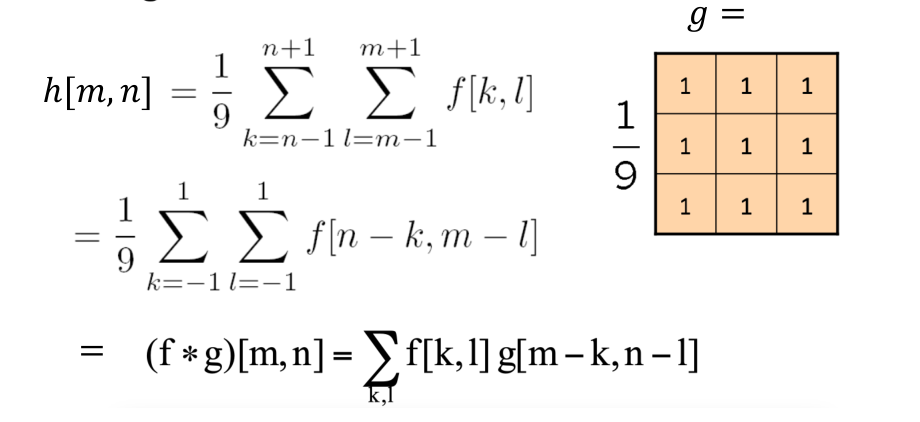
\includegraphics[scale=0.25]{figures/g.png}
    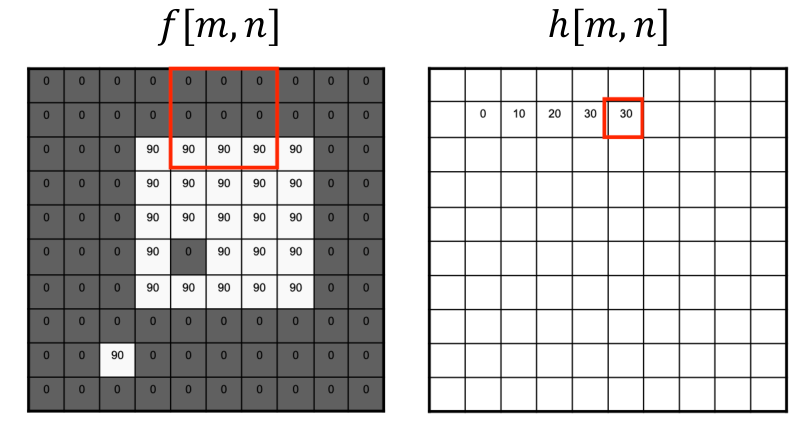
\includegraphics[scale=0.25]{figures/g2.png}
    \caption{Filtering examples.}
\end{figure}

\section{Non-linear Filtering}
\begin{itemize}
    \item 举例:\textbf{通过阈值(thresholding)进行二值化}:
    $$
    h(x,y) = 
    \begin{cases} 
    255 & \text{if } f(x,y) > T \\
    0   & \text{otherwise}
    \end{cases}
    $$
\end{itemize}

% --- Placeholder for image "BinarizationviaThresholding.png" ---
\begin{figure}[htbp]
    \centering
    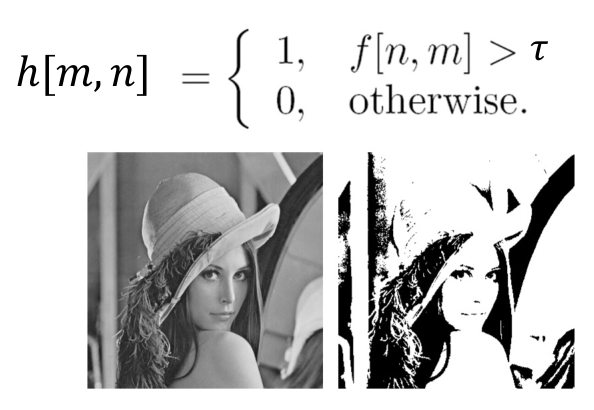
\includegraphics[scale=0.4]{figures/BinarizationviaThresholding.png}
    \caption{Binarization example.}
\end{figure}